% debut d'un fichier latex standard
\documentclass[a4paper,12pt,twoside]{article}
% Tout ce qui suit le symbole "%" est un commentaire
% Le symbole "\" désigne une commande LaTeX

% pour l'inclusion de figures en eps,pdf,jpg, png

\usepackage{subcaption}
\usepackage{wrapfig}
\usepackage{graphicx}
\usepackage{media9}
\usepackage[T1]{fontenc}
\usepackage{float}

\usepackage[utf8]{inputenc}
\usepackage[ngerman,english]{babel}
%\usepackage{graphicx}     % for \includegraphics
\usepackage{geometry}
\usepackage{svg}
\svgpath{{Pictures/}}
\usepackage{mathrsfs}

\usepackage{amsfonts}
% quelques symboles mathematiques en plus
\usepackage{amsmath}

% le tout en langue francaise
\usepackage[english]{babel}

% on peut ecrire directement les caracteres avec l'accent
%    a utiliser sur Linux/Windows (! dépend de votre éditeur !)
%\usepackage[utf8]{inputenc} % 
%\usepackage[latin1]{inputenc} % Pour Kile
\usepackage[T1]{fontenc}

%    a utiliser sur le Mac ???
%\usepackage[applemac]{inputenc}

% pour l'inclusion de liens dans le document 
\usepackage[colorlinks,bookmarks=false,linkcolor=blue,urlcolor=blue]{hyperref}
\paperheight=297mm
\paperwidth=210mm
\setlength{\parindent}{0pt}
\setlength{\parskip}{1em}

\setlength{\textheight}{235mm}
\setlength{\topmargin}{-1.2cm} % pour centrer la page verticalement
%\setlength{\footskip}{5mm}
\setlength{\textwidth}{16.5cm}
\setlength{\oddsidemargin}{0.0cm}
\setlength{\evensidemargin}{-0.3cm}

\pagestyle{plain}

% nouvelles commandes LaTeX, utilis\'ees comme abreviations utiles
\def \be {\begin{equation}}
\def \ee {\end{equation}}
\def \dd  {{\rm d}}

\newcommand{\mail}[1]{{\href{mailto:#1}{#1}}}
\newcommand{\ftplink}[1]{{\href{ftp://#1}{#1}}}

\newcommand{\betreuer}{Univ.\ Lektor Dipl.-Ing.\ Dr.techn.\ Stefan Gerhold}
\newcommand{\titel}{From the Gai Kapadia model to its empirical verification}
\newcommand{\untertitel}{Are more connections increasing the stability of the system ? \\ From the Gaussian point of view to the Power Law}
\newcommand{\autor}{Loïc Posta}
\newcommand{\telefon}{+41 78 685 06 97}
\newcommand{\email}{loic.posta@bluewin.ch}
\newcommand{\studium}{Physics, 6th Semester}
\newcommand{\abgabe}{28.02.2026}
\newcommand{\ausgabe}{28.02.2026}
\newcommand{\matrikel}{12505712}
%
% latex SqueletteRapport.tex      % compile la source LaTeX
% xdvi SqueletteRapport.dvi &     % visualise le resultat
% dvips -t a4 -o SqueletteRapport.ps SqueletteRapport % produit un PostScript
% ps2pdf SqueletteRapport.ps      % convertit en pdf

% pdflatex SqueletteRapport.pdf    % compile et produit un pdf

% ======= Le document commence ici ================================

\begin{document}

% --- Titlepage ---------------------------------------------------------------
\newgeometry{left=2.6cm,right=2.6cm,top=2.5cm,bottom=2.5cm}
\pagenumbering{arabic}
\setcounter{page}{1}

\begin{titlepage}
\setlength{\parindent}{0pt}
\thispagestyle{plain}

\begin{center}
    \large Technische Universität Wien\\
    \large Fakultät für Mathematik und Geoinformation\\
    \large Institut für Stochastik und Wirtschaftsmathematik\\
    \large Betreuer: \betreuer

    \vspace{1.0cm}
    \rule{\linewidth}{0.8pt}

    \vspace{0.9cm}
    {\LARGE \textbf{Seminar Arbeit}\par}

    \vspace{0.9cm}
    {\LARGE \textbf{\titel}\par}

    \vspace{0.25cm}
    % short centered divider (like in your photo)
    \rule{0.6cm}{0.5pt}\par

\vspace{0.25cm}
{\large\textit{\untertitel}\par}

    \vspace{0.9cm}
    \rule{\linewidth}{0.8pt}
\end{center}

\vspace{1.2cm}

% bottom info: left block (author & contact) / right block (dates)
\noindent
\begin{minipage}[t]{0.64\textwidth}
    \textbf{Eingereicht von:}\par
    \autor\par
    %Tel.: \telefon\par
    E-Mail: \email\par
    \studium\par
    Matriculation number: \matrikel
\end{minipage}
\hfill
\begin{minipage}[t]{0.32\textwidth}
    \raggedleft
    \textbf{Ausstellungsdatum:} \ausgabe\par
    \textbf{Submission date:} \abgabe
\end{minipage}

\vfill

% TU Wien logo bottom-right
\hfill
% If you have the logo as SVG, keep includesvg; otherwise use includegraphics with PDF/PNG.
\includesvg[width=0.32\textwidth]{TU_Wien-Logo.svg}
% 
\includegraphics[width=0.32\textwidth]{Pictures/TU_Wien-Logo.pdf}
\end{titlepage}
\restoregeometry
\clearpage
\tableofcontents
\clearpage

\pagenumbering{arabic}
% ----------------------------------------------------------------------------- 



\pagenumbering{arabic}
\setcounter{page}{3}
%\section{Abstract}
%Our financial systems are highly interconnected networks, which allows local shocks to propagate, and sometimes becoming large scale. Being able to predict the effects of local defaults on a whole network is a central question that lies between Graph Theory and Statistical Physics.

%In this paper, we describe those financial systems as graphs whose nodes represent economic agents and edges relations such as credit exposure.
%After introducing how a financial network can be described  with a graph, we introduce the Gai \& Kapadia model for direct contagion. That model, first introduced in 2010, describes the effects of a shock on a single agent and predicts percolation-like phase transitions between safe and likely to see a large contagion regimes. 

%With a simple Python program, we simulate scenarios for a network of $N=1000$ banks and confirm the predictions of the model, such as the existence of a contagion window depending on the average degree $z$ and two phase transitions for the average size of the cluster. Later, we study dynamics while varying the illiquidity and the capital buffer. Those experiments also allow us to discuss some guidance on how to limit the risks of propagation, for example with diversification and enough equity reserve.

%\newblock The full paper is available at : \footnote{\url{https://drive.google.com/file/d/15bNy6jpVY0VmZV3BFpKGe5L4Elyxav_s/view?usp=sharing}}.

\section{Introduction}
\label{sec:introduction}

The modern financial system is defined by a dense web of interconnected 
institutions whose mutual dependencies span the entire global economy. 
While this complexity was long considered a source of resilience --- 
allowing risk to be distributed across many participants --- the crisis 
of 2008 exposed its darker counterpart: that the same channels designed 
to absorb shocks can just as readily transmit them. The collapse of 
Lehman Brothers did not remain a local event; it propagated across 
balance sheets, asset classes, and national borders, demonstrating that 
systemic risk is fundamentally a collective phenomenon rather than the 
sum of individual failures. Understanding the mechanisms by which 
distress spreads through financial networks has since become a central 
preoccupation of both academic research and prudential regulation.

This paper builds upon the structural analysis of financial networks 
introduced by Clément Landry~\cite{landry2025}, and asks a sharper 
question: is the Gai-Kapadia model empirically correct? To answer 
this, we examine in depth the model proposed by Gai and 
Kapadia~\cite{gai2010}, which offers a rigorous and analytically 
tractable account of contagion in interbank networks, and confront its 
assumptions with evidence from real interbank markets.

The central question we set out to address is the following: does 
increased connectivity genuinely enhance the stability of a financial 
system? The Gai-Kapadia framework, we argue, rests implicitly on the 
assumption that interbank exposures follow a Gaussian distribution, 
arising naturally from the use of Erdős-Rényi random graphs. This 
assumption renders losses self-averaging and crises statistically 
improbable --- yet, when they occur, catastrophic. Empirical evidence, 
however, suggests that real interbank networks are better described by 
Power Law distributions and scale-free topologies, a distinction with 
profound consequences for how risk concentrates and how it propagates.

The paper proceeds as follows. Section~\ref{sec:network} introduces 
the necessary tools from graph theory and establishes the 
network-theoretic language used throughout. 
Section~\ref{sec:gaussian_vs_power} examines the statistical contrast 
between Gaussian and Power Law shock distributions, and motivates why 
this distinction is not merely technical but determinative of the 
system's qualitative behavior. Section~\ref{sec:gk_model} presents the 
Gai-Kapadia model in detail, with particular attention to its 
non-linear dynamics, phase transition structure, and the convergence 
properties of its finite-network simulations. 
Section~\ref{sec:comparison} compares the model's predictions against 
the empirical characteristics of real financial networks. Finally, 
Section~\ref{sec:conclusion} draws together the policy implications of 
our analysis and discusses the lessons that the 2008 crisis, and the 
subsequent Basel III reforms, offer for the calibration of theoretical 
models.
\newpage
\section{Network and Graph Theory}
\label{sec:network}
\subsection{From Isolation to Interdependence}

As established in the introduction, the 2008 financial crisis demonstrated 
that systemic risk cannot be understood by examining institutions in 
isolation. Banks borrow, lend, and share risk through dense webs of 
bilateral contracts, and it is precisely these linkages that transform a 
local failure into a global crisis. To model this structure rigorously, 
we turn to the language of graph theory, which provides both the 
vocabulary and the analytical tools needed to study how distress 
propagates through a financial system.

\begin{figure}[H]
    \centering
    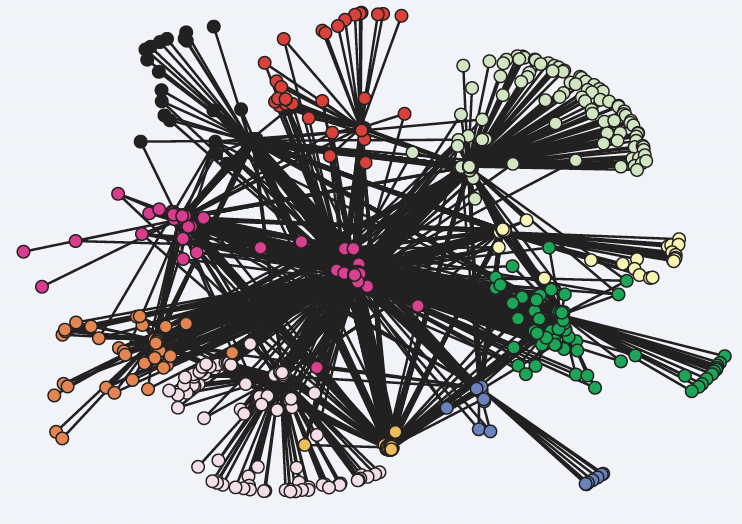
\includegraphics[width=0.6\linewidth]{austrian_bank_network.png}
    \vspace{0.3cm}
    \caption{The Austrian interbank network \cite{boss2004}. Each node represents a 
    financial institution, and each directed edge represents an exposure. 
    The heterogeneous degree distribution --- with a few highly connected 
    hubs and many peripheral nodes --- is characteristic of real-world 
    financial networks and motivates the Power Law analysis developed in 
    Section~\ref{sec:gaussian_vs_power}.}
    \label{fig:austrian_network}
\end{figure}

\subsection{Graph Theory Basics}

We represent a financial system as a directed graph $G(V, E)$, where:
\begin{itemize}
    \item \textbf{Vertices (Nodes)} $V$: represent economic agents such 
    as banks, insurance companies, or households.

    \item \textbf{Edges (Links)} $E$: represent financial relationships 
    between agents, such as loans, ownership stakes, or common asset 
    holdings. 
\end{itemize}

The connectivity structure of the graph is encoded in the 
\textbf{adjacency matrix} $A$, defined by:
\begin{equation}
    A_{ij} = 
    \begin{cases} 
        1 & \text{if there is a directed link from node } i 
          \text{ to node } j \\ 
        0 & \text{otherwise}
    \end{cases}
    \label{eq:adjacency}
\end{equation}

As a concrete example, consider a network of five nodes with the 
following adjacency matrix and edge set:
\[
A =
\begin{pmatrix}
0 & 1 & 0 & 0 & 0 \\
0 & 0 & 0 & 0 & 0 \\
0 & 0 & 0 & 1 & 1 \\
0 & 0 & 0 & 0 & 1 \\
0 & 1 & 0 & 0 & 0
\end{pmatrix}, 
\quad
V = \{1,2,3,4,5\}, 
\quad
E = \{1 \to 2,\; 3 \to 4,\; 5 \to 2,\; 4 \to 5,\; 3 \to 5\}
\]
While the in-degree of node 
    $i$, defined as $k_i^{\text{in}} = \sum_j A_{ji}$, counts the number 
    of creditors that have an exposure to $i$, the out-degree $k_i^{\text{out}} = \sum_j A_{ij}$ counts 
    the number of counterparties to which node $i$ is exposed.
\subsection{Types of Financial Relations}
\label{sec:types_relations}

Financial links vary considerably in nature, and recognizing this 
heterogeneity is essential for understanding both the richness of real 
interbank systems and the simplifications that theoretical models must 
make. We distinguish four levels of complexity.

\textbf{Directed and undirected graphs.} A loan from commercial bank 
$i$ to commercial bank $j$ creates an asymmetric exposure: $i$ bears 
the credit risk of $j$, but not vice versa. This is naturally 
represented as a \textbf{directed} graph, where $A_{ij} \neq A_{ji}$ 
in general. By contrast, a symmetric relationship such as a joint 
investment is better modeled as an \textbf{undirected} graph, in which 
$A_{ij} = A_{ji}$.

\textbf{Weighted graphs.} In most financial applications, the mere 
existence of a link is insufficient; its monetary value matters. We 
therefore assign a weight $\omega_{ij} \in \mathbb{R}_{+}$ to each 
edge, representing the size of the exposure. The binary adjacency 
matrix $A$ is then replaced by a weighted matrix $W$ with entries 
$W_{ij} = \omega_{ij}$, which allows the model to distinguish a 
small interbank loan from a systemically significant one.

\textbf{Different types of actors.} Real financial networks are not 
populated by identical institutions. A central bank occupies a 
structurally different position from a commercial bank: it acts as a 
lender of last resort, holds unique regulatory powers, and its failure 
— unlike that of a commercial bank — is not modeled as a credit event. 
Similarly, insurance companies, hedge funds, and clearing houses each 
interact with the network in distinct ways. Recognizing heterogeneity 
in node types is therefore important for accurately representing who 
can fail and how.

\textbf{Different types of relations.} Two institutions may be 
connected simultaneously through multiple channels: a direct lending 
relationship, a shared equity stake, and an exposure through 
derivatives contracts. Each type of relation transmits risk 
differently and responds differently to regulatory intervention. A 
complete model would represent each relation type as a separate layer 
of the network.

\begin{figure}[H]
    \centering
    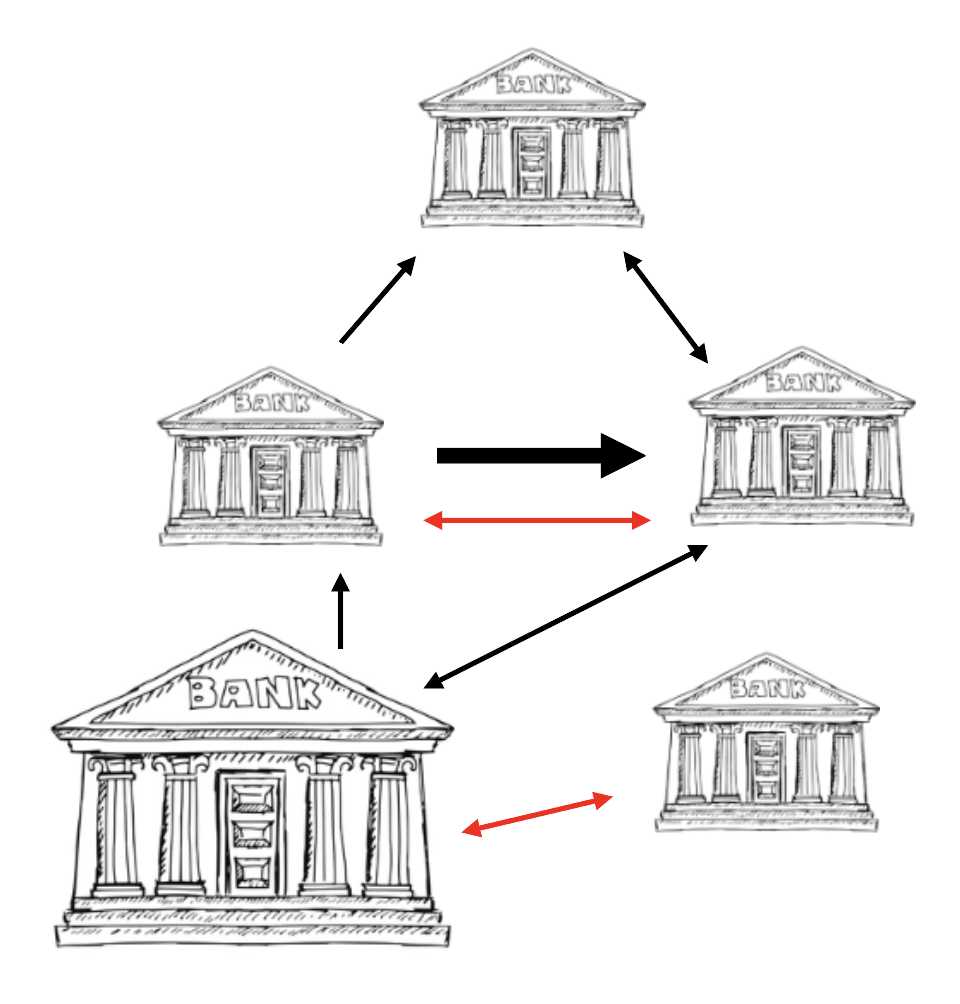
\includegraphics[width=0.42\linewidth]{graph.png}
    \caption{Illustration of a heterogeneous financial network. Arrows 
    indicate directed credit exposures: a directed edge from $i$ to $j$ 
    means that institution $i$ holds a claim on $j$ and bears the risk 
    of $j$'s default. Different edge colors represent distinct types of 
    contractual relationship. Node size distinguishes institution types: 
    larger nodes represent central banks or clearing houses, smaller 
    nodes represent commercial banks.}
    \label{fig:directed_graph}
\end{figure}
\vspace{-0.7cm}
\textit{Note:} The Gai-Kapadia model retains only the first two levels 
of this complexity. It represents the interbank system as a 
\textbf{weighted directed graph} with a single type of relationship 
(interbank lending) and a single type of actor (commercial banks). 
Central banks, derivatives, and equity cross-holdings are all 
abstracted away. This simplification makes the model analytically 
tractable, but it also means that the heterogeneity documented 
empirically in Section~\ref{sec:comparison} lies entirely outside its 
scope.
\vspace{-0.5cm}
\subsection{Quantitative Tools for Contagion}
\vspace{-0.5cm}
To characterize how vulnerable a network is to shock propagation, we 
rely on several structural metrics.

\textbf{Degree distribution} $P_k$: the probability that a randomly 
selected node has exactly $k$ connections. The shape of this 
distribution is critical: a highly concentrated distribution, with a 
few nodes of very high degree, indicates a system in which the failure 
of a single hub can immediately affect a large fraction of the network. 
As we will see in Section~\ref{sec:comparison}, this is precisely the 
topology observed in real interbank markets.

\textbf{Average degree} $z$: in a directed graph, the mean in-degree 
equals the mean out-degree, and both are equal to the average number of 
counterparties per institution:
\begin{equation}
    z = \sum_{j,k} j \cdot P_{jk} = \sum_{j,k} k \cdot P_{jk}
    \label{eq:avg_degree}
\end{equation}
This parameter plays a central role in the Gai-Kapadia model, where it 
serves as the primary control variable for the onset of systemic 
contagion.

\textbf{Clustering coefficient} $C$: the probability that two neighbors 
of a given node are also neighbors of each other. A high clustering 
coefficient implies that failures tend to be concentrated within 
densely connected subgraphs, which can amplify local shocks before they 
spread to the rest of the system.

\textbf{Average path length and the small-world property}: the average 
path length $\langle \ell \rangle$ measures the mean number of steps 
required to travel between any two nodes. Networks in which $\langle 
\ell \rangle$ is small relative to the total number of nodes are called 
\textit{small-world} networks. In such systems, a distress signal can 
reach any institution in only a few steps, meaning that local shocks 
become global almost instantaneously.
\subsection{A Physics Perspective}
\label{sec:physics_perspective}
The network-theoretic framework described above has a natural 
interpretation in terms of statistical mechanics, which we find 
particularly illuminating. The propagation of financial distress through 
an interbank network is formally analogous to a \textbf{percolation 
problem}~\cite{bardoscia2021}: nodes fail sequentially as the stress they face exceeds their 
capital buffer, and the question is whether the cascade reaches a 
macroscopic fraction of the system.

More precisely, the transition from a stable regime --- in which defaults 
remain localized --- to a systemic crisis is a \textbf{phase transition} 
in the sense of statistical mechanics. A single control parameter, the 
average degree $z$, plays the role of temperature: as it crosses a 
critical threshold, the global state of the system changes 
discontinuously. We will formalize this analogy in 
Section~\ref{sec:gk_model}, where the phase diagram of the 
Gai-Kapadia model is derived explicitly.

\begin{figure}[h]
    \centering
    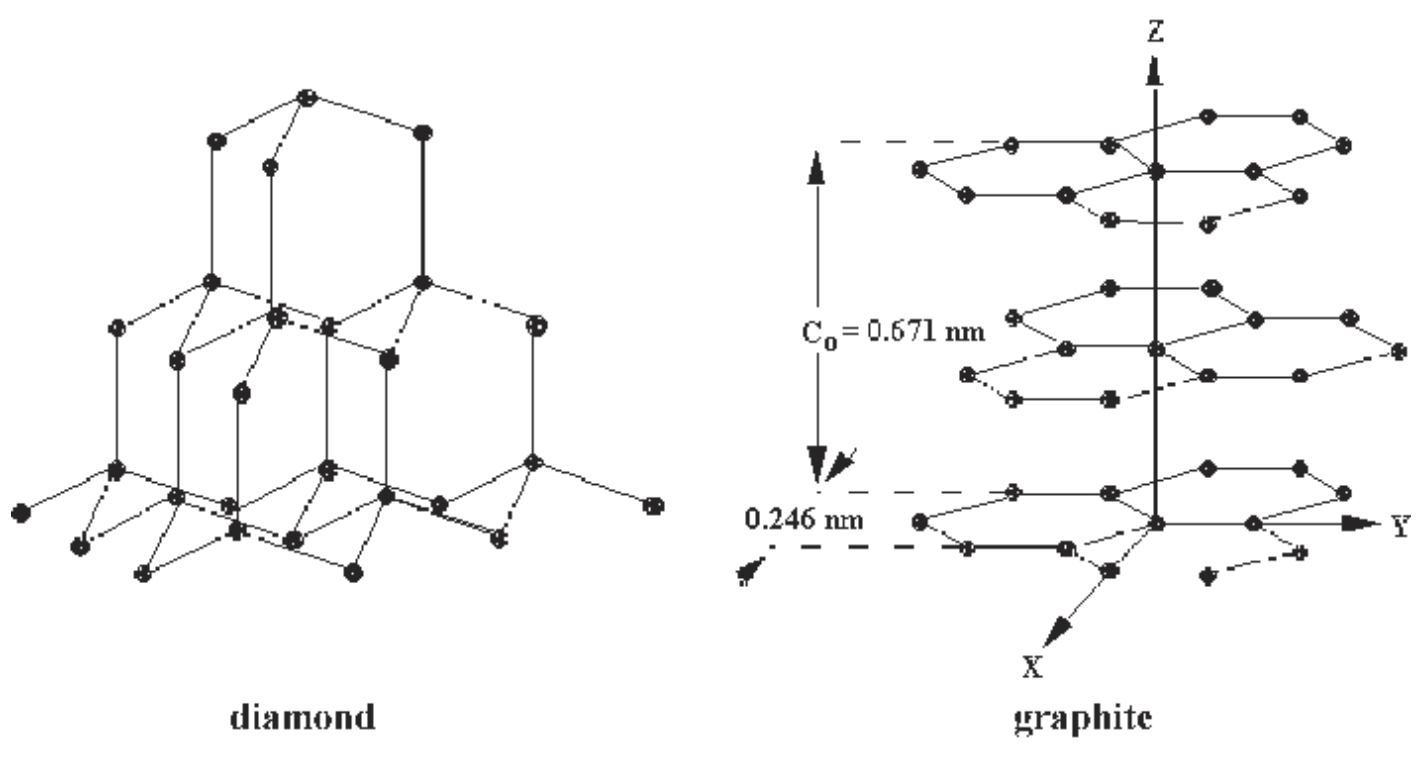
\includegraphics[width=0.5\linewidth]{network.png}
    \caption{Crystal structures of diamond (left) and graphite (right) 
as an analogy for financial network topology. In diamond, each carbon 
atom is connected to four others in a rigid three-dimensional lattice, 
creating a highly resilient structure. In graphite, atoms are strongly 
connected within layers but weakly connected across them, creating a 
direction-dependent fragility \cite{ceramic2006}. Similarly, the topology of interbank 
connections — not merely their number — determines whether a financial 
network absorbs or amplifies a shock.}
    \label{fig:contagion_cascade}
\end{figure}

\newpage
\section{Gaussian vs. Power-Law: The Nature of Shocks}
\label{sec:gaussian_vs_power}
\vspace{-0.5cm}

The architecture of a financial network determines the pathways along 
which distress can travel, but the outcome of a crisis depends equally 
on the nature of the initial shock. Before analyzing the mechanics of 
contagion in the Gai-Kapadia model, we must therefore ask a more 
fundamental question: what is the statistical character of the shocks 
to which a financial system is exposed? The answer to this question — 
whether extreme events are exponentially rare or structurally expected 
— has profound consequences for how we assess and regulate systemic 
risk.
\vspace{-0.6cm}
\subsection{Two Worlds: Mediocristan vs. Extremistan}
\vspace{-0.5cm}

Following the terminology introduced by Taleb~\cite{taleb2007}, we 
distinguish between two statistical regimes that lead to qualitatively 
different pictures of financial stability.

In the \textbf{Gaussian world} (thin tails), observations are 
concentrated around the mean and large deviations are exponentially 
suppressed. The system has a well-defined typical scale, and extreme 
events are so unlikely as to be practically impossible: a $10\sigma$ 
shock, for instance, would not be expected to occur even once over the 
lifetime of the universe. Risk in this regime is, in principle, 
manageable.

In the \textbf{Power-Law world} (heavy tails), the distribution decays 
slowly as a polynomial. Large shocks are rare, but they are not 
negligible — they are structurally built into the distribution. 
Crucially, if the tail exponent $\alpha$ satisfies $\alpha \leq 2$, the 
variance of the distribution is infinite, meaning that the system has 
no characteristic scale for disasters. Extreme events cannot be treated 
as anomalies; they must be treated as an expected feature of the 
environment.
\vspace{-0.2cm}

\begin{figure}[H]
    \centering
    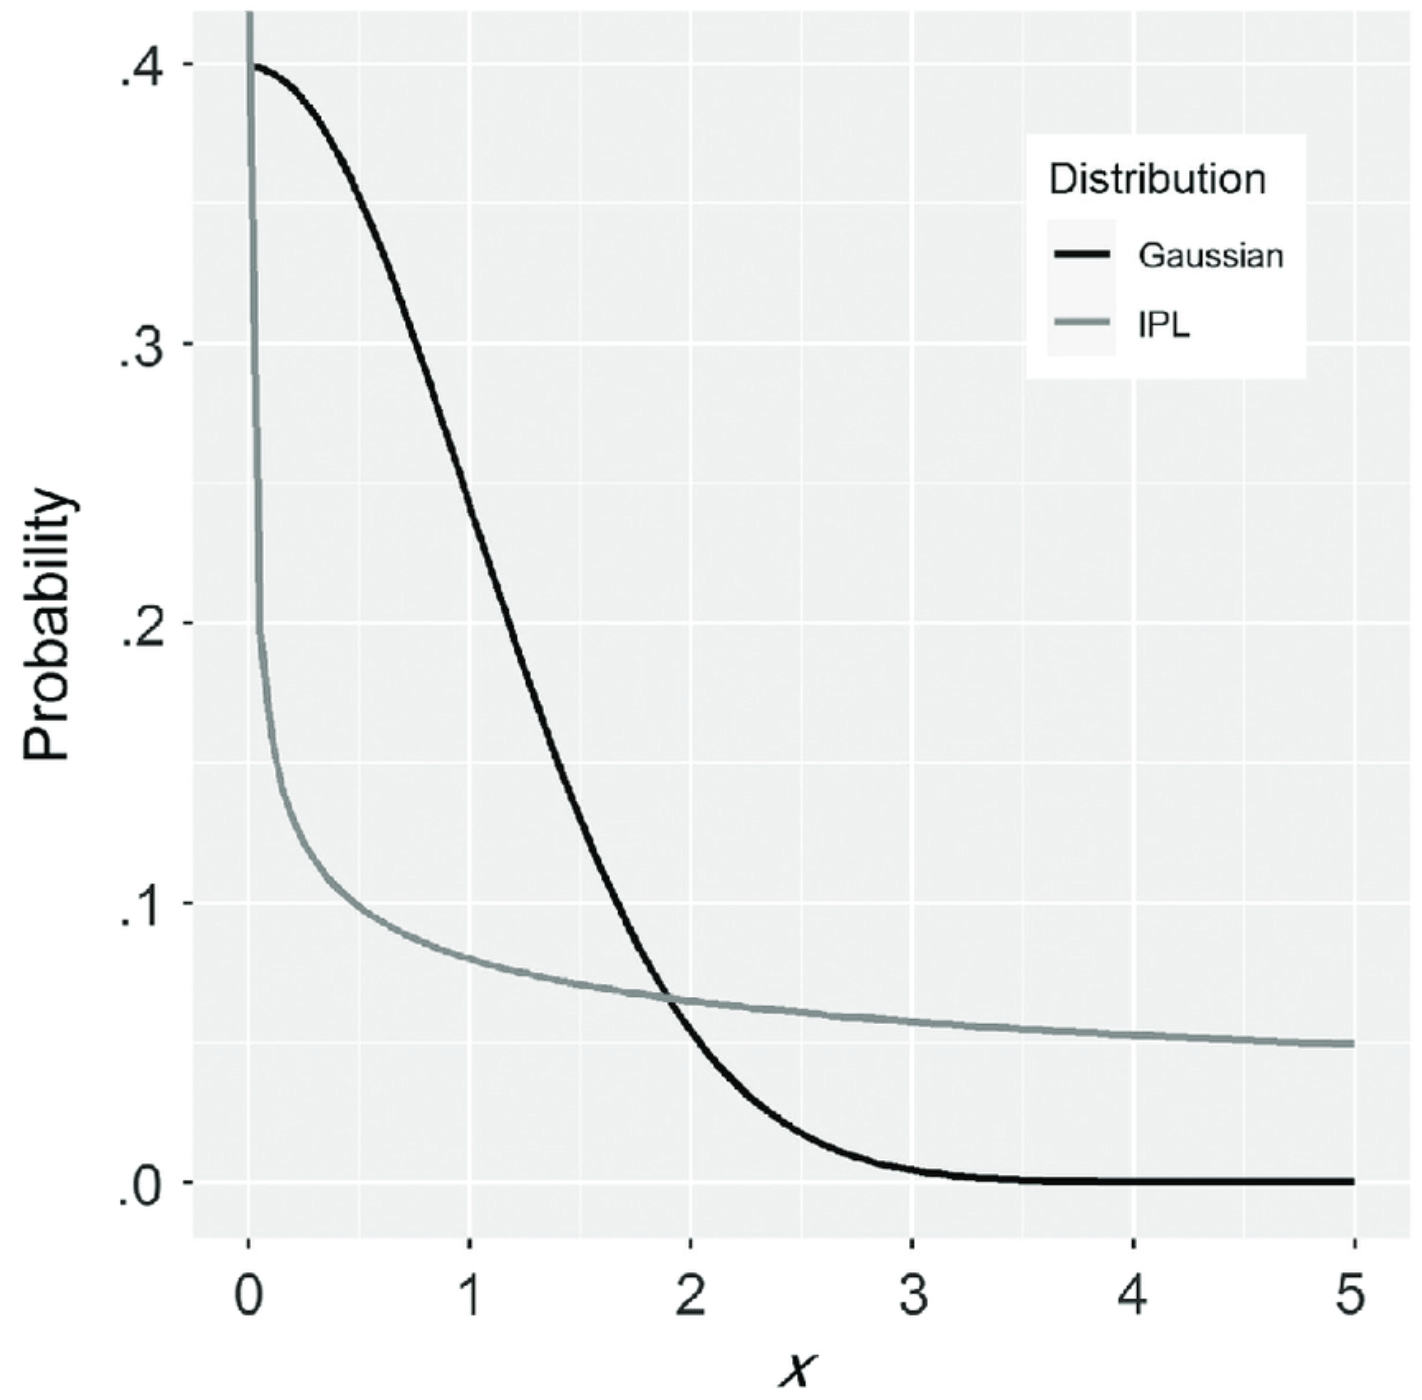
\includegraphics[width=0.44\linewidth]{gaussian_vs_power.png}
    \caption{Probability density functions of a Gaussian distribution 
    and an inverse power law (IPL). The Gaussian curve falls off 
    exponentially beyond the mean, while the power-law tail decays 
    slowly, assigning non-negligible probability to very large events. 
    This difference in tail behavior is the primary driver of the 
    contrasting stability properties discussed throughout this paper.}
    \label{fig:gaussian_vs_power}
\end{figure}
\vspace{-0.2cm}

\subsection{Mathematical Comparison}

The two regimes are distinguished by the form of their probability 
density functions (PDFs). Table~\ref{tab:gaussian_vs_power} summarizes 
the key properties.

\begin{table}[H]
\centering
\renewcommand{\arraystretch}{1.4}
\begin{tabular}{|l|c|c|}
\hline
\textbf{Feature} & \textbf{Gaussian (Normal)} & 
\textbf{Power Law (Pareto)} \\ \hline
\textbf{Equation} & 
    $\displaystyle f(x) = \frac{1}{\sigma\sqrt{2\pi}} 
    e^{-\frac{(x-\mu)^2}{2\sigma^2}}$ & 
    $\displaystyle f(x) = C x^{-\alpha}$ \\ \hline
\textbf{Mean} $\mathbb{E}[X]$ & 
    $\mu$ & 
    finite \; ($\alpha > 1$), \; 
    $\infty$ \; ($\alpha \leq 1$) \\ \hline
\textbf{Variance} $\mathrm{Var}(X)$ & 
    $\sigma^2$ & 
    finite \; ($\alpha > 2$), \;
    $\infty$ \; ($\alpha \leq 2$) \\ \hline
\textbf{Tail decay} & 
    Exponential (rapid) & 
    Polynomial (slow) \\ \hline
\textbf{Extreme events} & 
    Negligible & 
    Structurally present \\ \hline
\end{tabular}
\caption{Comparison of the Gaussian and Power Law (Pareto) 
distributions. Threshold values for the mean and variance refer to 
the PDF parameterization $f(x) = Cx^{-\alpha}$; the survival-function 
convention $P(X \geq x) \propto x^{-\alpha}$ shifts these thresholds 
by one~\cite{lteif2024}.}
\label{tab:gaussian_vs_power}
\end{table}

The choice of distributional assumption is not a technical detail; it 
determines the qualitative behavior of the entire system. A model 
calibrated under Gaussian assumptions will systematically underestimate 
the probability of tail events, and therefore the true extent of 
systemic risk. As we will see, this is precisely the limitation of the 
Gai-Kapadia framework.

\subsection{Implicit Gaussianity in the Gai-Kapadia Model}
\label{sec:implicit_gaussian}

The Gai-Kapadia model represents the interbank network as an 
\textbf{Erdős-Rényi random graph}, in which each pair of nodes is 
connected independently with probability $p$. For a network of $N$ 
banks, the degree of each node then follows a Poisson distribution with 
mean $\lambda = (N-1)p$. By the Central Limit Theorem, when $\lambda$ 
is large, this Poisson distribution converges to a Gaussian, so that 
the model effectively operates in a thin-tailed regime.

Three consequences follow directly from this construction. First, no 
institution accumulates a disproportionate number of counterparties: 
the degree distribution has an exponentially decaying tail, so that 
nodes with anomalously many connections are vanishingly unlikely. 
Second, interbank exposures are assumed to be independent and 
identically distributed (i.i.d.), so that the loss incurred by a bank 
upon the default of a neighbor is drawn from the same distribution 
regardless of which neighbor fails. Third, and most importantly, the 
aggregate loss faced by any given institution is a sum of i.i.d. 
random variables with finite variance. 
The CLT then guarantees that 
this sum is asymptotically Gaussian, making total losses 
\textit{self-averaging}: in the large-$N$ limit, the realized loss 
concentrates tightly around its expectation 
(see Appendix~\ref{sec:gaussian_proof}).

This self-averaging property is what makes the mathematics of the GK 
model tractable and elegant. It also, as we will argue in 
Section~\ref{sec:comparison}, makes it structurally blind to the 
fat-tailed reality of modern interbank markets, where the failure of a 
single highly connected institution can dominate the loss distribution 
of the entire system (see Appendix~\ref{sec:powerlaw_proof} for the 
contrasting Power-Law case).
\vspace{-0.8cm}
\section{The Gai-Kapadia Model: Robust yet Fragile}
\label{sec:gk_model}
\vspace{-0.5cm}

The seminal paper by Gai and Kapadia~\cite{gai2010} provides a 
cornerstone for the analytical study of financial contagion. Their 
central result is a paradox that challenges the naive intuition that 
more connectivity is always better: financial networks can be 
simultaneously \textbf{robust yet fragile}. The probability that any 
given shock triggers a systemic crisis may be low, but when contagion 
does occur, it is catastrophic in extent. Understanding the precise 
conditions under which this transition happens is the main objective 
of this section.
\vspace{-0.5cm}

\subsection{Modeling the Agent: The Bank Balance Sheet}
\label{sec:balance_sheet}
\vspace{-0.5cm}

The fundamental unit of the model is a bank, represented by its 
balance sheet. On the asset side, a bank holds outside assets 
(illiquid investments) and interbank assets (claims on other 
institutions). On the liability side, it carries outside liabilities 
(deposits and wholesale funding) and interbank liabilities (debts owed 
to counterparties), with the residual defined as net worth $w_i$.

A bank $i$ defaults when its net worth falls to zero, that is, when 
the losses it sustains from the default of its counterparties exceed 
its capital buffer $c_i$. Formally, if a fraction $q$ of its $z$ 
neighbors default and each bilateral exposure has value $\bar{p}$, 
bank $i$ defaults if:
\begin{equation}
    q \cdot z \cdot \bar{p} > c_i
    \label{eq:default_condition}
\end{equation}
This simple condition encodes the entire contagion mechanism: a bank 
survives if its capital is sufficient to absorb the losses from its 
defaulted counterparties, and fails otherwise, potentially triggering 
further defaults downstream.

\begin{figure}[H]
    \centering
    \vspace{-0.3cm}

    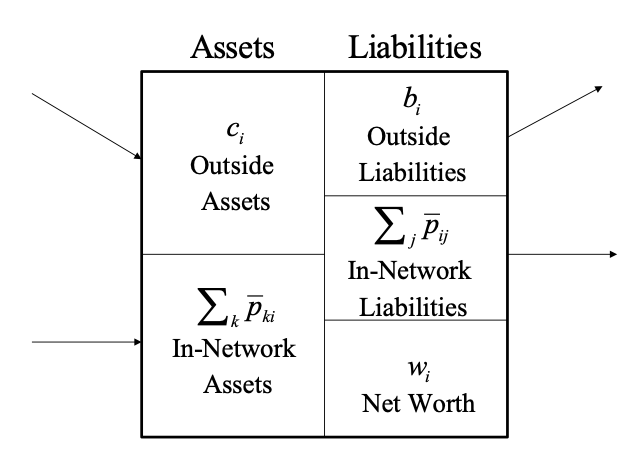
\includegraphics[width=0.42\linewidth]{bank_representation_gk.png}
    \vspace{-0.3cm}

    \caption{Stylized balance sheet of a bank in the Gai-Kapadia model. 
    Outside assets and interbank claims appear on the left; outside 
    liabilities, interbank obligations, and net worth on the right. 
    Default occurs when accumulated losses from counterparty failures 
    drive net worth $w_i$ to zero.}
    \label{fig:balance_sheet}
\end{figure}
\vspace{-1.5cm}

\subsection{Connectivity and the Topology of Risk}
\label{sec:connectivity}
    \vspace{-0.3cm}

The model is governed by three key quantities: the average degree $z$ 
(mean number of counterparties per bank), the \textit{frequency} $Y$ 
(the probability that a single initial failure triggers a systemic 
crisis, defined as more than 5\% of all banks failing), and the 
\textit{extent} (the total fraction of banks that ultimately default, 
conditional on a crisis occurring). Together, frequency and extent 
capture both how likely a crisis is and how severe it will be.

Numerical simulations of the model reveal that contagion is confined 
to a specific window of connectivity, which we can decompose into four 
qualitatively distinct regimes.

At low connectivity ($z < 2$), the network is too sparse for shocks 
to propagate. A defaulting bank has so few counterparties that its 
failure does not generate sufficient losses elsewhere to trigger 
secondary defaults, and the distress remains localized.

As connectivity increases toward $z \approx 3$, the network enters 
what we call the \textit{danger zone}. The system is now connected 
enough for a shock to travel across multiple hops, but not 
sufficiently diversified for individual banks to absorb the incoming 
losses. This is the regime of maximal contagion frequency: a single 
failure is most likely to cascade into a systemic crisis here.

At strong connectivity ($z > 5$), the picture reverses. Each bank now 
shares its interbank exposures across many counterparties, so the loss 
attributable to any single default is small relative to the receiving 
bank's capital buffer. Risk-sharing dominates, and the system becomes 
robust to small shocks.

Finally, beyond a critical threshold (indicated by the dashed line in 
Figure~\ref{fig:contagion_window}), contagion disappears entirely from 
the simulations. It is important to interpret this correctly: the drop 
of \textit{extent} to zero does not mean that crises become smaller. 
It means they cease to occur altogether, leaving the extent undefined. 
The system has crossed from the supercritical into the subcritical 
phase.
\vspace{-0.4cm}

\begin{figure}[H]
    \centering

    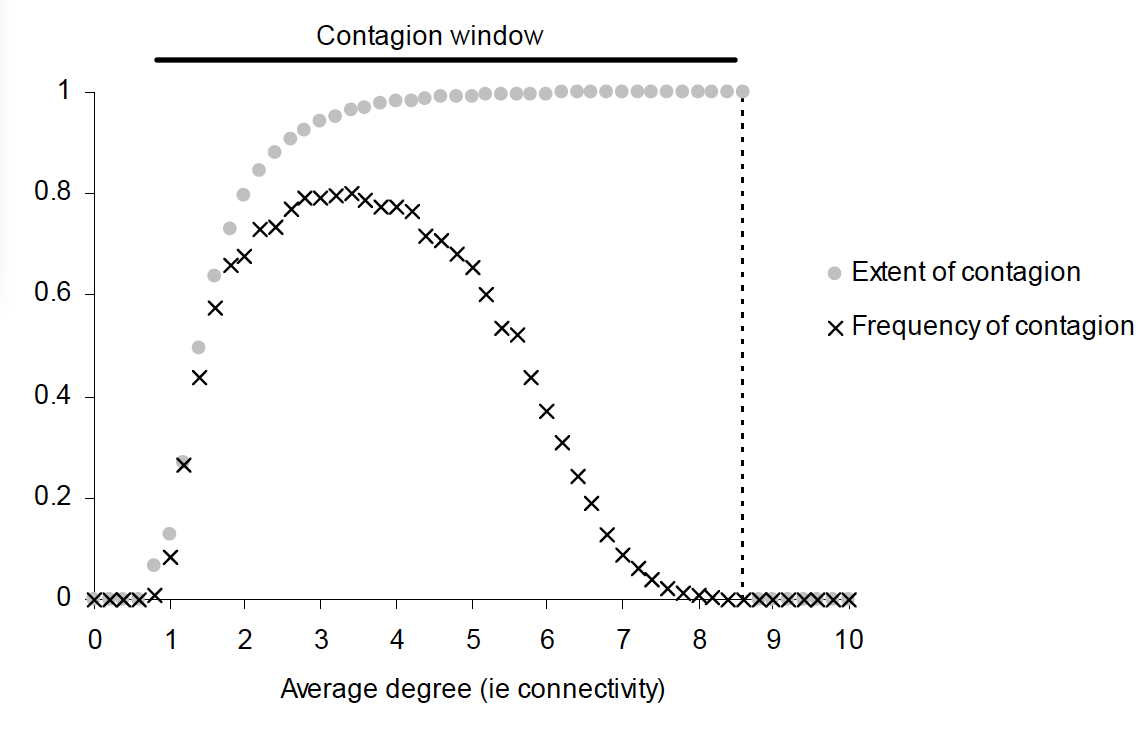
\includegraphics[width=0.56\linewidth]
    {type_of_contagion.png}
    \vspace{-0.3cm}

    \caption{Frequency and extent of contagion as a function of average 
    degree $z$, from Gai and Kapadia~\cite{gai2010}. The frequency of 
    contagion peaks near $z \approx 3$ before declining, while the 
    extent remains high within the contagion window. Beyond the dashed 
    threshold, both quantities drop to zero as the system enters the 
    subcritical regime.}
    \label{fig:contagion_window}
\end{figure}

\subsection{Non-Linearity, Phase Transitions, and the Knife-Edge 
Property}
\label{sec:nonlinearity}

Two features of the model deserve particular emphasis, as they 
have direct consequences for financial regulation.

The first is strict non-linearity. The relationship between 
connectivity and stability is not monotone: increasing $z$ from 2 to 
3 does not improve network safety but in fact maximizes the 
probability of global collapse. Standard regulatory intuitions — that 
more diversification is always better, or that incremental changes in 
lending requirements have proportional effects — are fundamentally 
misleading in this setting.

The second is what Gai and Kapadia call the \textit{knife-edge} 
property. Two initial shocks that are statistically indistinguishable 
can lead to radically different outcomes. At $z \approx 8$, for 
instance, an identical shock may have zero systemic effect in one 
simulation run, or trigger the total collapse of every institution in 
the network in another. The system's response is exquisitely sensitive 
to microscopic details of the network realization, making it 
essentially impossible to predict or prevent individual crises using 
conventional oversight tools.

From the perspective of statistical mechanics, this behavior is 
immediately recognizable as a \textbf{phase transition}. The average 
degree $z$ plays the role of a control parameter — analogous to 
temperature in a thermodynamic system — and the onset of systemic 
contagion corresponds to the system crossing a critical point. Just as 
water does not gradually become ice but undergoes a discontinuous 
change of state at a sharp temperature threshold, the financial network 
transitions abruptly from a stable subcritical phase to a 
contagion-dominated supercritical phase as $z$ crosses its critical 
value. The transition is not smooth; it is structural.

\begin{figure}[H]
    \centering
    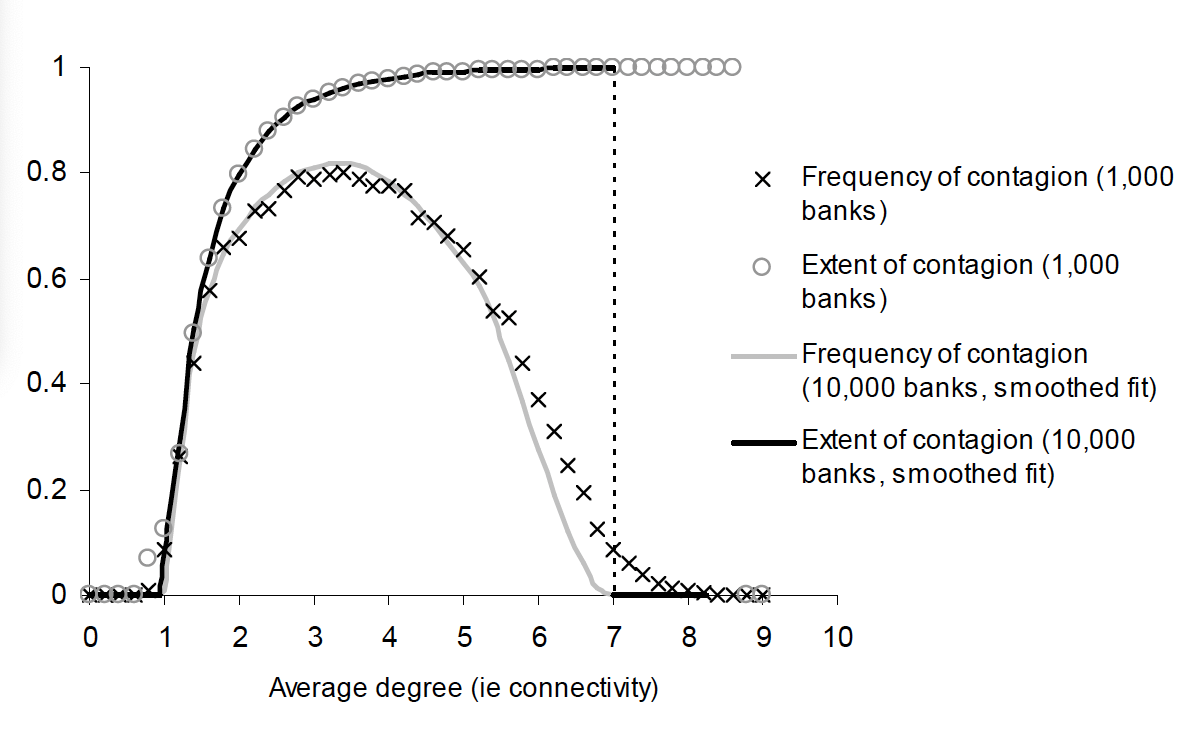
\includegraphics[width=0.6\linewidth]{convergence_contagion.png}
    \caption{Comparison of contagion simulations for $N = 1{,}000$ and 
    $N = 10{,}000$ banks. The near-identical results confirm that the 
    robust-yet-fragile property is a structural feature of the network 
    topology, not a finite-size artifact. As $N \to \infty$, the 
    Gaussian self-averaging argument of Section~\ref{sec:implicit_gaussian} 
    guarantees convergence to a deterministic limit.}
    \label{fig:convergence}
\end{figure}

\subsection{Structural Convergence and the $N \to \infty$ Limit}
\label{sec:convergence}

A natural concern about any simulation-based result is whether it 
reflects a genuine property of the model or merely an artifact of the 
finite system size. The Gai-Kapadia results are robust in this respect. 
As established in Section~\ref{sec:implicit_gaussian}, the loss 
distribution in the GK model is asymptotically Gaussian, and the 
Central Limit Theorem guarantees that aggregate losses concentrate 
around their mean as $N \to \infty$. The robust-yet-fragile property 
is therefore not a numerical accident but a structural consequence of 
the network's geometry.

This convergence is confirmed directly by comparing simulations at 
$N = 1{,}000$ and $N = 10{,}000$ banks, as shown in 
Figure~\ref{fig:convergence}. The frequency and extent curves are 
nearly indistinguishable across the two system sizes, establishing 
that the contagion window and the phase transition threshold are 
intrinsic properties of the interbank topology rather than 
finite-sample noise. The risk, in other words, is embedded in the 
geometry of the links themselves.

\section{Empirical Validation: From Mediocristan to Extremistan}
\label{sec:comparison}

The Gai-Kapadia model offers an analytically tractable account of 
financial contagion, but its predictive value ultimately depends on 
how faithfully it represents the structure of real interbank markets. 
In this section, we confront the model's Gaussian assumptions with 
empirical evidence from observed financial networks. The comparison 
reveals a fundamental mismatch: while the GK framework assumes a 
homogeneous, Erdős-Rényi topology, real interbank markets exhibit the 
heterogeneous, hub-dominated structure characteristic of scale-free 
networks. This distinction is not merely topological — it changes the 
qualitative nature of systemic risk.

\subsection{The Gaussian Perspective: Risk as a Statistical Average}
\label{sec:gaussian_perspective}

In the Gai-Kapadia framework, the financial system operates under the 
Law of Large Numbers. Because exposures are i.i.d. and the degree 
distribution is Poisson, aggregate risk is well-described by its mean, 
and the behavior of any individual institution is representative of 
the whole. Stability in this world arises from diversification: by 
spreading exposures across many similar counterparties, each bank 
reduces the impact of any single default to a manageable fraction of 
its capital buffer.

Fragility, correspondingly, is a threshold phenomenon. The system 
remains stable as long as the aggregate volume of shocks stays below 
the critical level required to exhaust the network's collective 
capital. Once that threshold is crossed, the phase transition described 
in Section~\ref{sec:nonlinearity} occurs, and defaults cascade 
globally. Below the threshold, however, the system is genuinely 
robust: shocks are absorbed by being spread thin across the network, 
and no single institution's failure is large enough to destabilize the 
whole.

This picture is internally consistent and mathematically elegant. Its 
limitation is that it assumes away the very feature of real financial 
networks that makes them most dangerous: extreme heterogeneity in the 
distribution of connections and exposures.

\subsection{The Power-Law Perspective: Risk as a Structural Property}
\label{sec:powerlaw_perspective}

Empirical studies of interbank networks consistently find that the 
degree distribution and the distribution of bilateral exposure sizes 
follow a Power Law rather than a Poisson distribution ~\cite{iori2008, 
boss2004}. Figures 
\ref{fig:contract_sizes}, \ref{fig:in_degree}, 
and~\ref{fig:out_degree} display log-log plots of contract size 
distributions and degree distributions from real interbank data. The 
approximately linear relationship on the log-log scale is the 
signature of a power law: $P(k) \sim k^{-\alpha}$, with estimated 
exponents in the range $\alpha \approx 1$ to $3$ depending on the 
market and the quantity measured.

In a scale-free network, the notion of an ``average'' institution 
loses its meaning. The system is instead defined by its hubs: a small 
number of highly connected institutions that intermediate a 
disproportionate share of total interbank activity. Major institutions 
of this type occupy a structurally different position from the 
periphery, and their behavior cannot be inferred from the mean.
\begin{figure}[H]
    \centering
    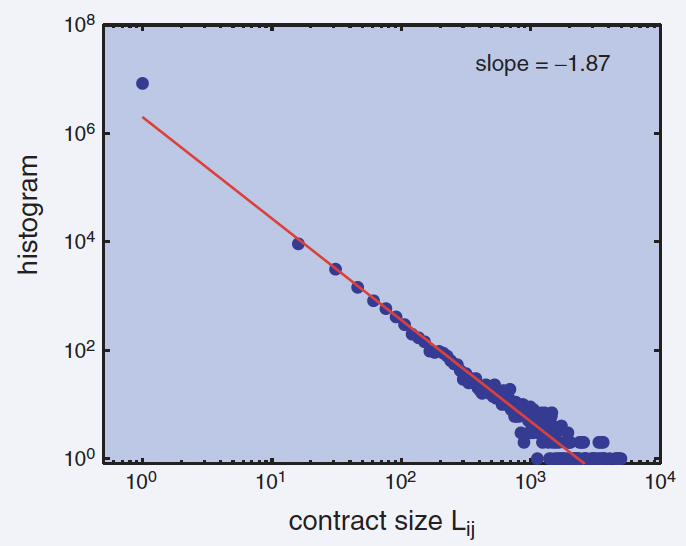
\includegraphics[width=0.75\linewidth]{magnitude_contracts.png}
    \caption{Log-log histogram of bilateral contract sizes $L_{ij}$ in 
    an empirical interbank network. The approximately linear slope of 
    $-1.87$ on the log-log scale confirms a power-law distribution of 
    exposure sizes, implying that extremely large bilateral contracts 
    — absent from Erdős-Rényi models — are a structural feature of 
    real markets.}
    \label{fig:contract_sizes}
\end{figure}

\begin{figure}[H]
    \centering
    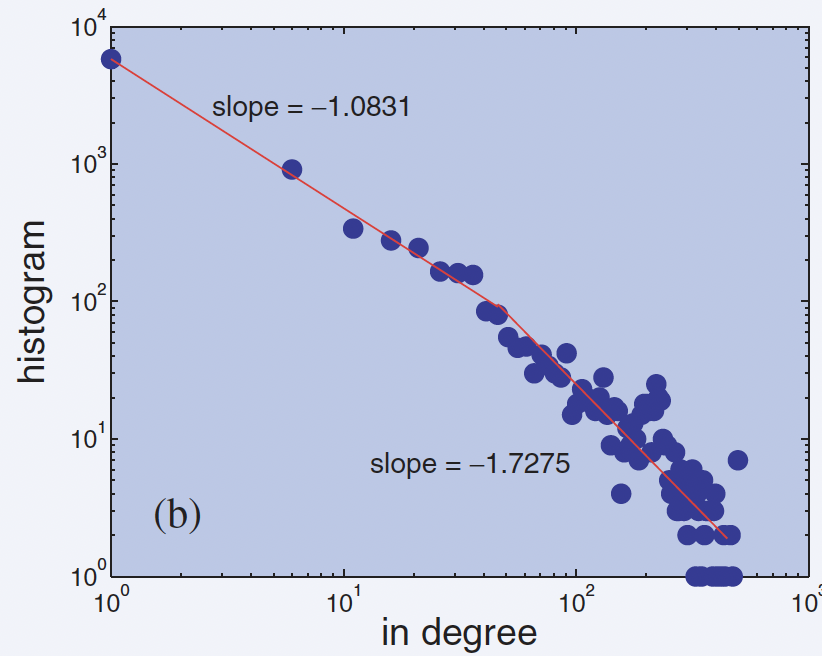
\includegraphics[width=0.7\linewidth]{real_life_creditors.png}
    \caption{Log-log histogram of in-degrees (number of creditors) in 
    the empirical interbank network. The two-regime power-law fit, with 
    slopes $-1.08$ for small degrees and $-1.73$ for large degrees, 
    indicates the presence of a small number of institutions with a 
    disproportionately large number of creditors — the hubs of the 
    lending network.}
    \label{fig:in_degree}
\end{figure}
\vspace{-1cm}
\begin{figure}[H]
    \centering
    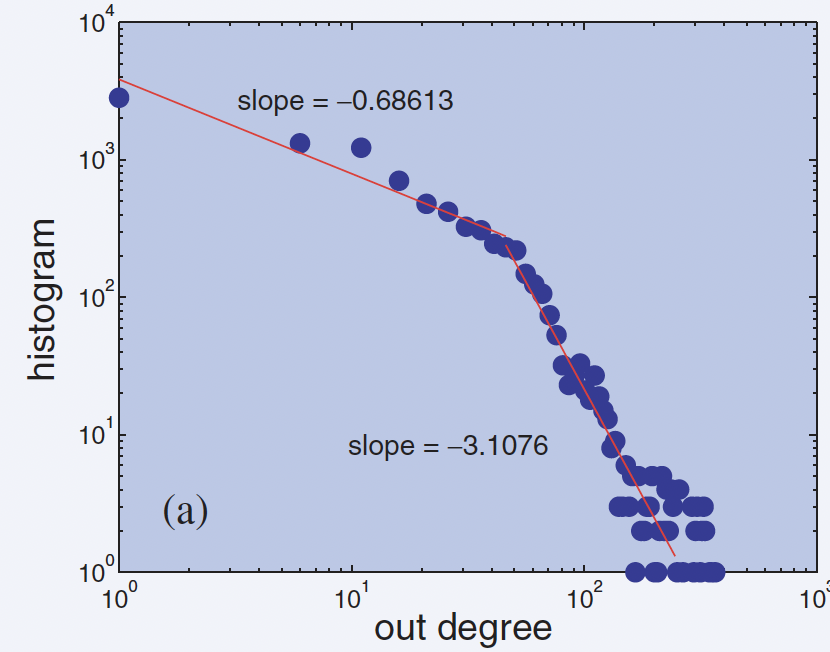
\includegraphics[width=0.7\linewidth]{real_life_debtors.png}
    \caption{Log-log histogram of out-degrees (number of debtors) in 
    the empirical interbank network. The slope of $-0.69$ in the bulk 
    and $-3.11$ in the tail reflects a highly skewed distribution of 
    borrowing activity, with a small number of institutions acting as 
    dominant borrowers.}
    \label{fig:out_degree}
\end{figure}



This topology generates a fundamentally different pattern of 
robustness and fragility. Against random failures — the default of a 
randomly selected bank — scale-free networks are remarkably resilient, 
because the vast majority of nodes are peripheral and their failure 
has negligible systemic impact. Against targeted failures, however, 
the network is acutely vulnerable. The collapse of a single hub 
propagates instantly to the large number of institutions directly 
exposed to it, and the resulting cascade can dominate the loss 
distribution of the entire system.

A further consequence is that the supercritical phase — in which a 
path to global contagion exists — is not confined to a window of 
intermediate connectivity, as in the GK model. Because hubs maintain 
permanent high-degree connections throughout the network, the 
topological conditions for systemic propagation are structurally 
present at all times. The financial system is, in this sense, always 
on the edge of criticality.

\subsection{Summary Comparison}
\label{sec:summary_comparison}

Table~\ref{tab:comparison} summarizes the structural differences 
between the two frameworks.

\begin{table}[H]
\centering
\renewcommand{\arraystretch}{1.5}
\begin{tabular}{|l|p{5cm}|p{5cm}|}
\hline
\textbf{Feature} & \textbf{Gaussian World (GK)} & 
\textbf{Power-Law World (Scale-Free)} \\ \hline
\textbf{Network topology} & 
    Erdős-Rényi (homogeneous) & 
    Scale-free (hub-dominated) \\ \hline
\textbf{Robustness mechanism} & 
    Diversification across many similar counterparties & 
    Absorption capacity of high-degree hubs \\ \hline
\textbf{Fragility mechanism} & 
    Aggregate shock volume exceeds capital threshold & 
    Targeted failure of a single hub \\ \hline
\textbf{Shock propagation} & 
    Distributed and attenuated by spreading & 
    Amplified at hubs; absorbed at periphery \\ \hline
\textbf{Supercritical phase} & 
    Confined to intermediate connectivity window & 
    Structurally present at all connectivity levels \\ \hline
\textbf{Physics analogy} & 
    Sharp phase transition (discontinuous) & 
    Permanent criticality (self-organized) \\ \hline
\end{tabular}
\caption{Structural differences in systemic risk between the Gaussian 
(Gai-Kapadia) and Power-Law (scale-free) frameworks.}
\label{tab:comparison}
\end{table}
\newpage
\subsection{The Central Lesson}
\label{sec:takeaway}

The comparison above points to a conclusion that is both 
mathematically precise and practically important. In a Gaussian world, 
systemic risk is described by the mean: the behavior of the average 
institution is representative of the whole, and risk management 
reduces to controlling aggregate exposure volumes. In a Power-Law 
world, risk is dominated by the extremes: the fate of the system rests 
on the tail of the distribution, and the behavior of a handful of 
dominant institutions is more consequential than the combined activity 
of all the rest.

Systemic risk is therefore not simply a scaled-up version of 
idiosyncratic risk. It is a structural property of the network, 
determined by the topology of connections rather than the average 
characteristics of individual nodes. A regulatory framework that 
monitors only the ``average'' bank — or that assumes exposures are 
drawn from a thin-tailed distribution — is structurally blind to the 
most dangerous configurations that real financial networks can 
exhibit.\footnote{For an accessible visual treatment of why power laws 
are pervasive in complex systems, see Muller, D. \cite{veritasium2024}. While not a primary academic 
source, it provides useful geometric intuition for the hub-and-spoke 
structure discussed here.}

\newpage
\section{Conclusion and Outlook}
\label{sec:conclusion}
\subsection{Final Synthesis: The Connectivity Paradox}
For decades, the prevailing economic intuition was that increasing connectivity would necessarily make the financial system more stable through better risk-sharing. Our analysis of the Gai-Kapadia model and Power-Law dynamics challenges this simplistic view. 

While connectivity improves stability \textbf{locally} by allowing banks to diversify their exposures, it creates \textbf{systemic fragility} once certain topological thresholds are crossed. This highlights a critical lesson: economic mechanisms rarely behave in a linear fashion. More connectivity does not always imply more stability; instead, it can create "super-highways" for contagion.

\subsection{Key Policy Implications}
The results of this study suggest that monetary and regulatory policies must shift their focus from individual health to \textbf{network health}:
\begin{itemize}
    \item \textbf{Network Supervision:} It is not enough to monitor a bank's internal balance sheet. Regulators must supervise the \textit{structure} of the network to prevent the formation of dangerous contagion channels.
    \item \textbf{Accounting for Thresholds:} Policy-making must account for non-linear effects. A small change in interbank interest rates or lending requirements can push the system across a phase transition boundary, moving it from a stable state to a supercritical one.
\end{itemize}

\subsection{Outlook: The Reality of Capital Buffers}
\label{sec:outlook}

The 2008 financial crisis provides a direct empirical test of the 
model's parameters. The capital buffer used in theoretical simulations 
of the GK model is typically set at approximately 4\% — a figure that, 
in retrospect, proved inadequate to contain the cascading failures 
observed in practice. The collapse of Lehman Brothers, whose leverage 
left it with minimal effective capital against its interbank 
exposures, triggered precisely the domino dynamics the model predicts.

The regulatory response was the Basel III framework, which 
substantially raised minimum capital requirements relative to its 
predecessor. Where Basel II had set total capital requirements at 
approximately 8\% of risk-weighted assets, Basel III raised the 
effective floor to roughly 13\%, incorporating a capital conservation 
buffer and systemic risk surcharges for globally significant 
institutions\cite{boss2004, basel2013}.

\begin{figure}[H]
    \centering
    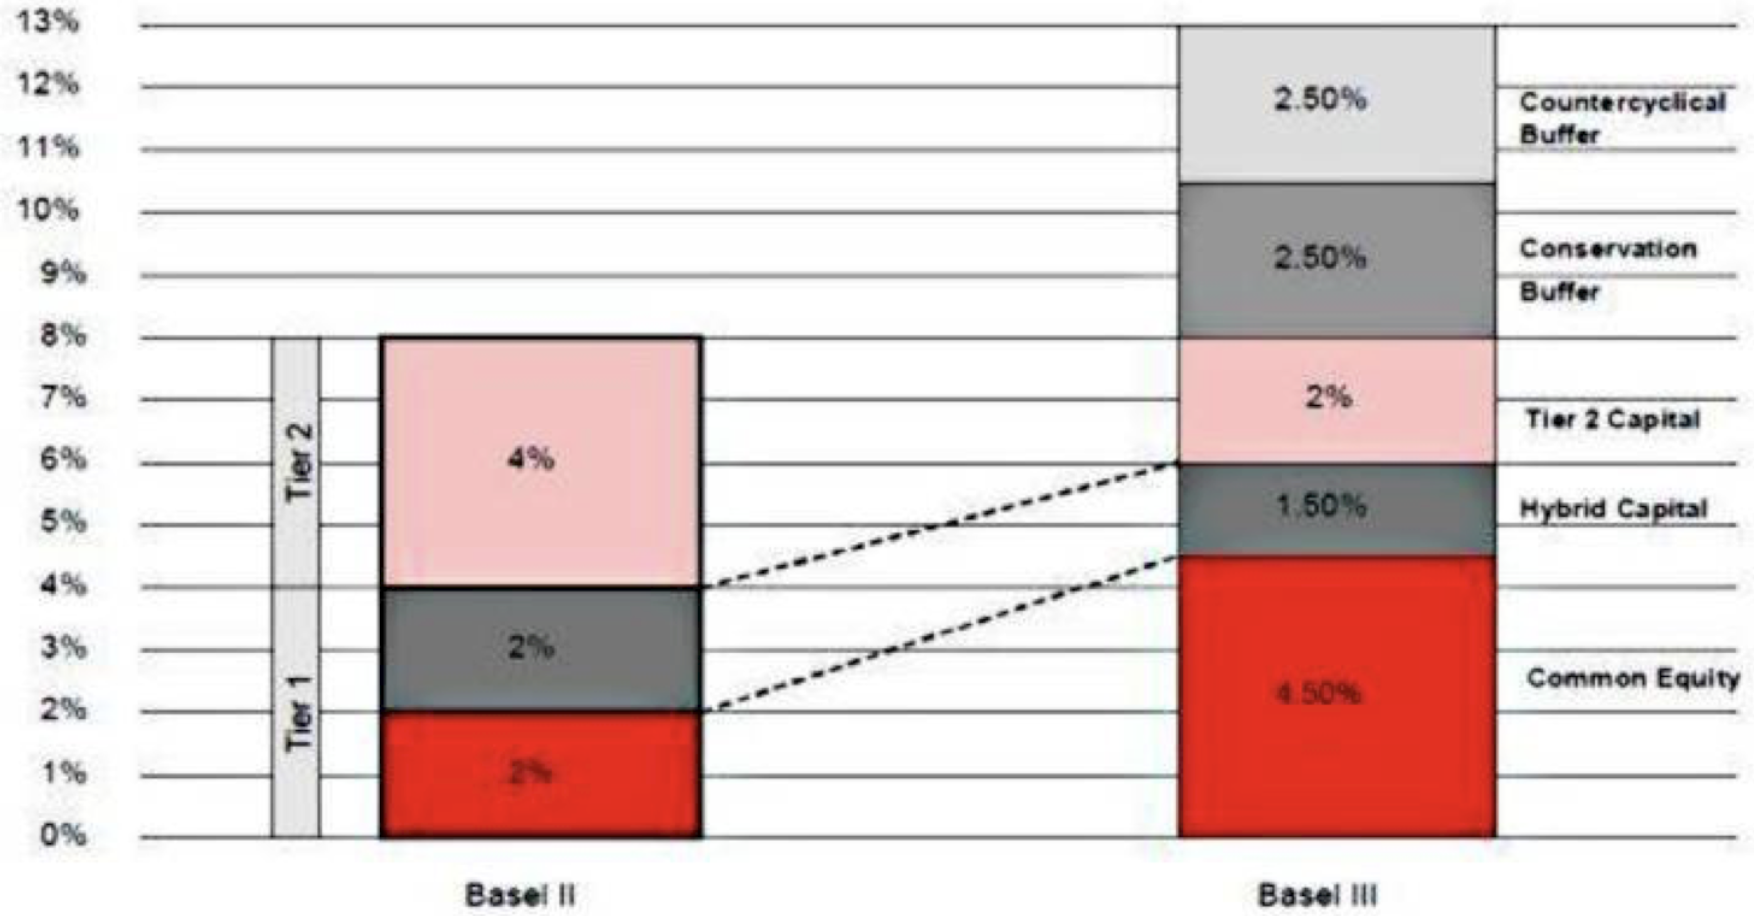
\includegraphics[width=0.65\linewidth]{basel3.png}
    \caption{Capital requirement structure under Basel III~\cite{basel2013}. The total 
    requirement of approximately 13\% is composed of a minimum Tier 1 
    capital ratio, a capital conservation buffer, and an additional 
    surcharge for globally systemically important institutions (G-SIIs). 
    Compared to the 8\% floor under Basel II, this represents a 
    structural shift in the regulatory approach to systemic risk.}
    \label{fig:basel3}
\end{figure}

In the language of the model, raising capital requirements corresponds 
to increasing the default threshold of each node: a larger shock is 
required to trigger any individual failure, which shifts the system 
away from the fragile intermediate connectivity regime identified in 
Section~\ref{sec:connectivity}. To reduce systemic fragility, one must 
either reduce the density of dangerous connections through 
de-leveraging, or increase the resilience of the nodes themselves 
through higher capital. Basel III chose the latter path, and 
Figure~\ref{fig:basel3} illustrates the resulting buffer structure.

The financial system is a complex dynamical system. Managing it 
effectively requires treating it as one — not as a collection of 
independent institutions, but as an interconnected network whose 
global properties emerge from the topology of its links. The tools of 
network theory and statistical mechanics, applied here through the 
lens of the Gai-Kapadia model, offer a rigorous foundation for that 
endeavor.

%-----------------------------------------------------------
\newpage
\begin{thebibliography}{99}

\bibitem{landry2025}\label{landry}
C.~Landry,
\newblock ``Representing Financial Networks as Graphs
and Studying Direct Contagion Using the
Gai--Kapadia Model,''
\newblock Seminar Arbeit, Institut f\"{u}r Stochastik und 
Wirtschaftsmathematik, Technische Universit\"{a}t Wien, 2025.

\bibitem{gai2010}\label{GK}
P.~Gai and S.~Kapadia,
\newblock ``Contagion in financial networks,''
\newblock {\em Proceedings of the Royal Society A: Mathematical, 
Physical and Engineering Sciences}, vol.~466, no.~2120, 
pp.~2401--2423, 2010.
\newblock Available at: \url{https://www.jstor.org/stable/25706352}
\newblock [Accessed: 17 Nov. 2025]

\bibitem{boss2004}\label{network_topology}
M.~Boss, H.~Elsinger, M.~Summer, and S.~Thurner,
\newblock ``Network topology of the interbank market,''
\newblock {\em Quantitative Finance}, vol.~4, no.~6, pp.~677--684, 
2004.
\newblock DOI: \url{https://doi.org/10.1080/14697680400020325}
\newblock [Accessed: Jan. 2026]

\bibitem{bardoscia2021}\label{physics_of_financial}
M.~Bardoscia, P.~Barucca, S.~Battiston, F.~Caccioli, G.~Cimini,
D.~Garlaschelli, F.~Saracco, T.~Squartini, and G.~Caldarelli,
\newblock ``The Physics of Financial Networks,''
\newblock {\em arXiv preprint arXiv:2103.05623}, 2021.
\newblock Available at: \url{https://arxiv.org/abs/2103.05623}
\newblock [Accessed: 10 Oct. 2025]

\bibitem{ceramic2006}
\newblock ``Are ceramic nanofilms a soft matter?,''
\newblock 2006.
\newblock [Referenced for the structural analogy between crystal 
lattice topology and financial network connectivity, 
Section~\ref{sec:physics_perspective}.]

\bibitem{taleb2007}
N.~N.~Taleb,
\newblock {\em The Black Swan: The Impact of the Highly Improbable},
\newblock Random House, New York, 2007.

\bibitem{lteif2024}
G.~Lteif,
\newblock ``Gaussian Distributions vs Power Laws: Your Ultimate Guide 
to Making Sense of Natural and Social Phenomena,''
\newblock \textit{SoftwareDominos}, April 2024.
\newblock Available at: \url{https://softwaredominos.com/home/science-technology-and-other-fascinating-topics/gaussian-distributions-vs-power-laws-your-ultimate-guide-to-making-sense-of-natural-and-social-phenomena/}
\newblock [Accessed: Jan. 2026]

\bibitem{iori2008}\label{italian}
G.~Iori, G.~De~Masi, O.~V.~Precup, G.~Gabbi, and G.~Caldarelli,
\newblock ``A network analysis of the Italian overnight money market,''
\newblock {\em Journal of Economic Dynamics and Control}, vol.~32, 
no.~1, pp.~259--278, 2008.
\newblock [Accessed: Jan. 2026]

\bibitem{veritasium2024}\label{veritasium}
D.~Muller [Veritasium],
\newblock ``You've (Likely) Been Playing The Game of Life Wrong,''
\newblock YouTube, 2024.
\newblock Available at: \url{https://www.youtube.com/watch?v=HBluLfX2F_k}
\newblock [Accessed: Jan. 2026]
\bibitem{basel2013}
% Auteur(s) à compléter
\newblock ``Supervision of Financial Institutions Revisited: 
The Transition from Basel I to Basel III. A Critical Appraisal 
of the Newly Established Regulatory Framework in Response to 
the Credit Crunch,''
\newblock {\em % journal/revue à compléter}, 
% vol., pp., année à compléter.
\bibitem{zdeborova2025}\label{lenka}
L.~Zdeborová,
\newblock ``Introduction to Data Science,''
\newblock Course notes, École Polytechnique Fédérale de Lausanne 
(EPFL), 2025.

\bibitem{wald1944}
A.~Wald,
\newblock ``On Cumulative Sums of Random Variables,''
\newblock {\em The Annals of Mathematical Statistics}, vol.~15, no.~3, 
pp.~283--296, 1944.
\newblock Available at: \url{https://doi.org/10.1214/aoms/1177731235}
\newblock [Accessed: 07 Mar. 2026]

\bibitem{gnedenko1954}
B.~V.~Gnedenko and A.~N.~Kolmogorov,
\newblock {\em Limit Distributions for Sums of Independent Random 
Variables},
\newblock Addison-Wesley, Cambridge, MA, 1954.

\end{thebibliography}
\newpage
\appendix
\section{Mathematical Foundations of the Gaussian Regime}
\label{sec:annex}

This appendix provides the mathematical foundations underlying the 
arguments developed in the main text. We first derive \cite{zdeborova2025} the self-consistency 
equation that governs the onset of contagion in the Gai-Kapadia model, 
then prove that the loss distribution is asymptotically Gaussian in the 
Erdős-Rényi setting, and finally show why this Gaussian approximation 
breaks down when exposures follow a Power Law.

%------------------------------------------------------------------
\subsection{The Self-Consistency Equation and the Phase Transition}
\label{sec:self_consistency}

The fraction $q$ of defaulted banks is not a free parameter of the 
model — it is determined endogenously by the network structure. A bank 
$i$ defaults if the losses it sustains from its defaulted counterparties 
exceed its capital buffer $c_i$. Given that bank $i$ has $k_i$ 
counterparties and each bilateral exposure has normalized value 
$\bar{p}$, the default condition is:
\begin{equation}
    \sum_{j=1}^{k_i} \mathbf{1}_{\{j \,\text{defaults}\}} \cdot \bar{p} 
    > c_i
    \label{eq:default_condition_annex}
\end{equation}
Let $q$ denote the probability that a randomly chosen bank has 
defaulted. On an Erdős-Rényi graph with average degree $z$, the number 
of defaulted neighbors of bank $i$ follows a Binomial$(k_i, q)$ 
distribution. For large $k_i$, this is approximated by Poisson$(zq)$. 
Bank $i$ defaults if the number of defaulted neighbors exceeds the 
threshold $\lfloor c_i / \bar{p} \rfloor$. Averaging over the degree 
distribution and the distribution of capital buffers, the fraction of 
defaulted banks satisfies the \textbf{self-consistency equation}:
\begin{equation}
    q = \rho + (1 - \rho) \sum_{k=0}^{\infty} P_k 
    \sum_{m > c/\bar{p}} \binom{k}{m} q^m (1-q)^{k-m}
    \label{eq:self_consistency}
\end{equation}
where $\rho$ is the fraction of banks hit by the initial shock and 
$P_k$ is the degree distribution. This equation may admit multiple 
solutions. A solution $q \approx \rho$ (close to the initial shock 
size) corresponds to the \textbf{subcritical phase}: contagion does 
not spread beyond the initially affected banks. A solution $q \gg \rho$ 
corresponds to the \textbf{supercritical phase}: a small initial shock 
propagates to a macroscopic fraction of the network. The onset of 
contagion — the phase transition identified in 
Section~\ref{sec:nonlinearity} — corresponds precisely to the 
bifurcation point at which a second, large solution to 
equation~\eqref{eq:self_consistency} first appears.

%------------------------------------------------------------------
\subsection{Formal Proof of the Gaussian Limit}
\label{sec:gaussian_proof}

We now prove that, under the Erdős-Rényi assumption, the individual 
loss $L_i$ is asymptotically Gaussian and that aggregate losses are 
self-averaging.

\textbf{Structural assumptions.}
\begin{itemize}
    \item The network is an Erdős-Rényi random graph. The degree $k_i$ 
    of each node follows a Poisson distribution with mean $\lambda = zp$:
    \[
        P(k_i = k) = \frac{\lambda^k e^{-\lambda}}{k!}
    \]
    \item Interbank exposures $w_{ij}$ are i.i.d.\ with finite mean 
    $\mu$ and finite variance $\sigma^2$.
    \item Each neighbor defaults independently with probability $q$, 
    so the per-neighbor loss variable is:
    \[
        X_j = w_{ij} \cdot \mathbf{1}_{\{j\,\text{defaults}\}}
    \]
\end{itemize}

\textbf{Step 1: Moments of $X_j$.}
Since default occurs with probability $q$ independently of the exposure 
size:
\begin{align}
    \mathbb{E}[X_j] &= q\mu \label{eq:EX}\\
    \mathbb{E}[X_j^2] &= q(\sigma^2 + \mu^2) \label{eq:EX2}\\
    \text{Var}(X_j) &= \mathbb{E}[X_j^2] - (\mathbb{E}[X_j])^2 
    = q\sigma^2 + q(1-q)\mu^2 \label{eq:VarX}
\end{align}

\textbf{Step 2: Wald's Identity~\cite{wald1944} for the compound sum.}
The total loss of bank $i$ is a compound Poisson sum:
\[
    L_i = \sum_{j=1}^{k_i} X_j
\]
where $k_i \sim \text{Pois}(\lambda)$ is independent of the $X_j$. 
Applying Wald's Identity:
\begin{align}
    \mathbb{E}[L_i] &= \mathbb{E}[k_i]\,\mathbb{E}[X_j] 
    = \lambda q\mu \label{eq:ELi}
\end{align}
For the variance, we use the law of total variance:
\begin{equation}
    \text{Var}(L_i) = \mathbb{E}[k_i]\,\text{Var}(X_j) + 
    (\mathbb{E}[X_j])^2\,\text{Var}(k_i)
    \label{eq:VarLi_general}
\end{equation}
Substituting the Poisson property $\text{Var}(k_i) = \mathbb{E}[k_i] 
= \lambda$ and equation~\eqref{eq:VarX}:
\begin{equation}
    \text{Var}(L_i) = \lambda\bigl[q\sigma^2 + q(1-q)\mu^2 + 
    (q\mu)^2\bigr] = \lambda\bigl[q\sigma^2 + q\mu^2\bigr]
    = \lambda q(\sigma^2 + \mu^2)
    \label{eq:VarLi}
\end{equation}

\textbf{Step 3: CLT convergence for individual losses.}
Since $L_i$ is a sum of i.i.d.\ terms $X_j$ with a random number of 
summands, we apply the CLT for compound Poisson processes. As 
$\lambda \to \infty$:
\begin{equation}
    \frac{L_i - \mathbb{E}[L_i]}{\sqrt{\text{Var}(L_i)}} 
    \xrightarrow{d} \mathcal{N}(0,1)
    \label{eq:CLT_individual}
\end{equation}

\textbf{Step 4: Self-averaging of aggregate losses.}
Consider the system-wide average loss $\bar{L} = \frac{1}{N}
\sum_{i=1}^{N} L_i$. Since the $L_i$ are identically distributed with 
mean $\mu_L = \lambda q\mu$ and variance $\sigma_L^2 = \lambda q
(\sigma^2 + \mu^2)$, the Law of Large Numbers gives:
\begin{equation}
    \bar{L} \xrightarrow{a.s.} \mu_L = \lambda q\mu 
    \quad \text{as } N \to \infty
    \label{eq:self_averaging}
\end{equation}
This is the self-averaging property: in the large-$N$ limit, the 
realized aggregate loss concentrates deterministically around its 
expectation, and fluctuations vanish. The probability of an extreme 
aggregate loss event decays as:
\begin{equation}
    \mathbb{P}\!\left(\bar{L} > \mu_L + t\right) \sim 
    \exp\!\left(-\frac{t^2}{2\sigma_L^2/N}\right) 
    \quad \text{as } N \to \infty
    \label{eq:tail_decay}
\end{equation}
confirming that tail events are exponentially suppressed. The 
Gai-Kapadia model is therefore structurally incapable of generating 
the fat-tailed aggregate loss distributions observed in real financial 
crises.

%------------------------------------------------------------------
\subsection{When the CLT Fails: The Power Law Regime}
\label{sec:powerlaw_proof}

We now show that replacing the finite-variance assumption on $w_{ij}$ 
with a Power-Law distribution invalidates both the CLT and the 
self-averaging result.

Suppose $w_{ij}$ follows a Pareto distribution with tail exponent 
$\alpha$:
\begin{equation}
    f_W(w) = \frac{\alpha\, x_{\min}^\alpha}{w^{\alpha+1}}, 
    \quad w \geq x_{\min},\quad \alpha > 0
    \label{eq:pareto}
\end{equation}
For $1 < \alpha \leq 2$, the mean $\mathbb{E}[w_{ij}]$ is finite but 
the variance $\text{Var}(w_{ij})$ is infinite. For $\alpha \leq 1$, 
even the mean diverges. In either case, the conditions required for 
equation~\eqref{eq:VarX} to hold are violated.

The standard CLT requires finite variance. When $\text{Var}(w_{ij}) = 
\infty$, the Generalized Central Limit Theorem applies instead ~\cite{gnedenko1954}: the 
normalized sum of i.i.d.\ Pareto variables converges not to a Gaussian 
but to a \textbf{Lévy $\alpha$-stable distribution} $S_\alpha$, 
characterized by power-law tails of the same exponent $\alpha$.

The practical consequence is stark. In the Gaussian regime, 
self-averaging holds and aggregate losses concentrate around the mean:
\begin{equation}
    \bar{L} \xrightarrow{a.s.} \mu_L \quad \text{(Gaussian world)}
\end{equation}
In the Power-Law regime, the aggregate loss is instead dominated by 
its largest term:
\begin{equation}
    \bar{L} \approx \frac{1}{N} \max_{i} L_i 
    \quad \text{(Power-Law world)}
\end{equation}
This result — that the maximum single loss dominates the total — is a 
direct consequence of the heavy tail. It means that the failure of one 
sufficiently large institution can account for a macroscopic share of 
the system's total stress, regardless of how many other institutions 
are present. Self-averaging fails completely, and the Law of Large 
Numbers provides no protection.

This mathematical shift furnishes the rigorous explanation for the 
empirical observation that motivated this paper: a single institution 
— Lehman Brothers — could destabilize a global financial system that 
appeared statistically stable under Gaussian assumptions. The system 
was not stable; it was merely operating in a regime where the dominant 
risk was invisible to the tools being used to measure it.

\end{document} %%%% THE END %%%%
